
\documentclass[a4paper]{article}
\usepackage{times}
\usepackage[utf8]{inputenc}
\usepackage{selinput}
\usepackage{upquote}
\usepackage[margin=2cm, rmargin=4cm, tmargin=3cm]{geometry}
\usepackage{tcolorbox}
\usepackage{xspace}
\usepackage[french]{babel}
\usepackage{url}
\usepackage{hyperref}
\usepackage{fontawesome5}
\usepackage{marginnote}
\usepackage{ulem}
\usepackage{tcolorbox}
\usepackage{graphicx}
%\usepackage[top=Bcm, bottom=Hcm, outer=Ccm, inner=Acm, heightrounded, marginparwidth=Ecm, marginparsep=Dcm]{geometry}


\newtcolorbox{Example}[1]{colback=white,left=20pt,colframe=slideblue,fonttitle=\bfseries,title=#1}
\newtcolorbox{Solutions}[1]{colback=white,left=20pt,colframe=green,fonttitle=\bfseries,title=#1}
\newtcolorbox{Conseils}[1]{colback=white,left=20pt,colframe=slideblue,fonttitle=\bfseries,title=#1}
\newtcolorbox{Warning}[1]{colback=white,left=20pt,colframe=warning,fonttitle=\bfseries,title=#1}

\setlength\parindent{0pt}

  %Exercice environment
  \newcounter{exercice}
  \newenvironment{Exercice}[1][]
  {
  \par
  \stepcounter{exercice}\textbf{Question \arabic{exercice}:} (\faClock \enskip \textit{#1})
  }
  {\bigskip}
  

% Title
\newcommand{\titre}{\begin{center}
  \section*{Algorithmes et Pensée Computationnelle}
\end{center}}
\newcommand{\cours}[1]
{\begin{center} 
  \textit{#1}\\
\end{center}
  }


\newcommand{\exemple}[1]{\newline~\textbf{Exemple :} #1}
%\newcommand{\attention}[1]{\newline\faExclamationTriangle~\textbf{Attention :} #1}

% Documentation url (escape \# in the TP document)
\newcommand{\documentation}[1]{\faBookOpen~Documentation : \href{#1}{#1}}

% Clef API
\newcommand{\apikey}[1]{\faKey~Clé API : \lstinline{#1}}
\newcommand{\apiendpoint}[1]{\faGlobe~Url de base de l'API \href{#1}{#1}}

%Listing Python style
\usepackage{color}
\definecolor{slideblue}{RGB}{33,131,189}
\definecolor{green}{RGB}{0,190,100}
\definecolor{blue}{RGB}{121,142,213}
\definecolor{grey}{RGB}{120,120,120}
\definecolor{warning}{RGB}{235,186,1}

\usepackage{listings}
\lstdefinelanguage{texte}{
    keywordstyle=\color{black},
    numbers=none,
    frame=none,
    literate=
           {é}{{\'e}}1
           {è}{{\`e}}1
           {ê}{{\^e}}1
           {à}{{\`a}}1
           {â}{{\^a}}1
           {ù}{{\`u}}1
           {ü}{{\"u}}1
           {î}{{\^i}}1
           {ï}{{\"i}}1
           {ë}{{\"e}}1
           {Ç}{{\,C}}1
           {ç}{{\,c}}1,
    columns=fullflexible,keepspaces,
	breaklines=true,
	breakatwhitespace=true,
}
\lstset{
    language=Python,
	basicstyle=\bfseries\footnotesize,
	breaklines=true,
	breakatwhitespace=true,
	commentstyle=\color{grey},
	stringstyle=\color{slideblue},
  keywordstyle=\color{slideblue},
	morekeywords={with, as, True, False, Float, join, None, main, argparse, self, sort, __eq__, __add__, __ne__, __radd__, __del__, __ge__, __gt__, split, os, endswith, is_file, scandir, @classmethod},
	deletekeywords={id},
	showspaces=false,
	showstringspaces=false,
	columns=fullflexible,keepspaces,
	literate=
           {é}{{\'e}}1
           {è}{{\`e}}1
           {ê}{{\^e}}1
           {à}{{\`a}}1
           {â}{{\^a}}1
           {ù}{{\`u}}1
           {ü}{{\"u}}1
           {î}{{\^i}}1
           {ï}{{\"i}}1
           {ë}{{\"e}}1
           {Ç}{{\,C}}1
           {ç}{{\,c}}1,
    numbers=left,
}

\newtcbox{\mybox}{nobeforeafter,colframe=white,colback=slideblue,boxrule=0.5pt,arc=1.5pt, boxsep=0pt,left=2pt,right=2pt,top=2pt,bottom=2pt,tcbox raise base}
\newcommand{\projet}{\mybox{\textcolor{white}{\small projet}}\xspace}
\newcommand{\optionnel}{\mybox{\textcolor{white}{\small Optionnel}}\xspace}
\newcommand{\advanced}{\mybox{\textcolor{white}{\small Pour aller plus loin}}\xspace}
\newcommand{\auto}{\mybox{\textcolor{white}{\small Auto-évaluation}}\xspace}


\usepackage{environ}
\newif\ifShowSolution
\NewEnviron{solution}{
  \ifShowSolution
	\begin{Solutions}{\faTerminal \enskip Solution}
		\BODY
	\end{Solutions}
  \fi}


  \usepackage{environ}
  \newif\ifShowConseil
  \NewEnviron{conseil}{
    \ifShowConseil
    \begin{Conseils}{\faLightbulb \quad Conseil}
      \BODY
    \end{Conseils}

    \fi}

    \usepackage{environ}
  \newif\ifShowWarning
  \NewEnviron{attention}{
    \ifShowWarning
    \begin{Warning}{\faExclamationTriangle \quad Attention}
      \BODY
    \end{Warning}

    \fi}
  

%\newcommand{\Conseil}[1]{\ifShowIndice\ \newline\faLightbulb[regular]~#1\fi}


\usepackage{array}
\newcolumntype{C}[1]{>{\centering\let\newline\\\arraybackslash\hspace{0pt}}m{#1}}

\begin{document}
% Change the following values to true to show the solutions or/and the hints
\ShowSolutiontrue
\ShowConseiltrue
\titre
\cours{Programmation orientée objet - Exercices avancés}

Le but de cette séance est de se familiariser avec un paradigme de programmation couramment utilisé: la Programmation Orientée Objet (POO). Ce paradigme consiste en la définition et en l'interaction avec des briques logicielles appelées \lstinline{Objets}. Dans les exercices suivants, nous manipulerons des objets, aborderons les notions de classe, méthodes, attributs et encapsulation. Au terme de cette séance, vous serez en mesure d'écrire des programmes mieux structurés.
Afin d'atteindre ces objectifs, nous utiliserons principalement le langage \lstinline{Java} qui offre une panoplie d'outils pour mieux comprendre ce paradigme de programmation.

Le code présenté dans les énoncés se trouvent sur Moodle, dans le dossier \lstinline{Ressources}.

\section{Manipulation de graphes en POO (Java)}

%\subsection{Introduction}
% TODO: Cette sous-section devrait être convertie en introduction. Les questions sont intéressantes. Toutefois, elles perdent de leur utilité si les étudiants n'ont pas accès aux réponses de façon immédiate. Il serait préférable de les reformuler et de les utiliser comme rappel avant de commencer à faire les exercices suivants.


%Ici, on cherche à pousser votre réflexion sur le processus de conception de classes pour implémenter un concept existant en dehors de la programmation.
%Pour cela, il faut se placer du point de vue de l'utilisateur pour savoir ce dont il aurait besoin. 
%Il faut aussi savoir de quoi est constitué le concept que l'on cherche à implémenter. C'est-à-dire, pour utiliser une analogie, les différentes briques qui sont utilisées pour construire le mur qui est votre objet final.

Cette partie constitue un rappel sur la notion de graphe orienté. Avant de traiter les exercices de cette partie, veuillez répondre aux questions suivantes:
    \begin{enumerate}
        \item Quels sont les composantes d'un \lstinline{graphe orienté} ?
        \item Combien de classes sont nécessaires pour représenter un graphe orienté ainsi que toutes ses composantes?
        \item Sachant que vous avez une classe qui représente les \lstinline{arêtes} et que les \lstinline{sommets} sont représentés par des chaînes de caractères. Quels pourraient être les attributs de la classe \lstinline{graph}.
    \end{enumerate}

Maintenant que vous avez une idée des attributs de la classe \lstinline{graph} à définir, déterminer quelles méthodes sont nécessaires au fonctionnement de cet objet. Pour ce faire, vous pouvez répondre aux questions suivantes:
    \begin{enumerate}
    \item Est-ce que l'utilisateur aura besoin de modifier l'objet une fois celui-ci aura été initialisé ?
    \item Est-ce que l'utilisateur aura besoin de vérifier l'état de l'objet (existence d'attributs, vérification de valeurs...) ou de certaines parties de l'objet ?
    \end{enumerate}

\begin{conseil}
   % Un conseil
   N'hésitez pas à revenir sur le cours de la semaine 7 (algorithmes de graphes) disponible sur Moodle.
\end{conseil}
    
Voici les réponses aux questions posées ci-dessus. 

\textbf{Certaines questions peuvent avoir plus d'une réponse étant donné qu'il existe plusieurs manières de représenter un graphe en programmation. }
    %\lstinputlisting{solutions/fichier.java}
    \begin{enumerate}
    \item \begin{enumerate}
          \item Les \lstinline{sommets}.
          \item Les \lstinline{arêtes}.
          \item Le \lstinline{poids} de chaque arête.
          \end{enumerate}
    \item Il faut 2 classes ( ou 3 si on cherche à avoir plus d'informations dans les sommets):
        \begin{enumerate}
        \item Une classe \lstinline{Edge} qui va représenter les arêtes.
        \item Une classe \lstinline{Graph}.
        \end{enumerate}
    \item La classe \lstinline{Graph} va avoir 2 attributs: un ensemble contenant les \lstinline{sommets} et un autre ensemble contenant les \lstinline{arêtes} de celui-ci.
    
%    \item Les réponses à cette partie sont courtes mais assez essentielles pour savoir quelles méthodes coder:
 %       \begin{enumerate}
       % \item Oui, l'utilisateur voudra sûrement rajouter des \lstinline{arêtes}, des \lstinline{sommets} ou potentiellement changer le poids d'une \lstinline{arête}. Il faut donc lui laisser cette possibilité
       % \item Les graphs sont souvent accompagnés par des algorithmes de recherche, par exemple l'algorithme de Kruskal pour les \lstinline{weighted graphs}. Il est donc utile de pouvoir identifier si un \lstinline{sommet} ou une \lstinline{arête} sont des composants de l'instance.
       % \item Certaines méthodes pourraient avoir un code très long si on ne segmentarise pas leur contenu. Cela peut entraver la relecture de votre code par vous ou par un tiers. 
        
       % De plus dans un cadre d'optimisation, il faut éviter un maximum la redondance du code. Il est donc de bonne pratique de définir des méthodes qui vont éviter cela dans une classe.
  %      \end{enumerate}
    \end{enumerate}

%\subsection{Partie 2}
% TODO: Edge doit être mis au singulier pour éviter qu'ils ne confondent l'objet à son instance.

Le code de la classe \lstinline{Edge} est fourni dans le dossier ressources sur Moodle.
Utiliser le fichier \lstinline{Main.java} dans le dossier \lstinline{Code} sur Moodle pour effectuer des tests. Une fois exécuté, il devrait afficher:\\

    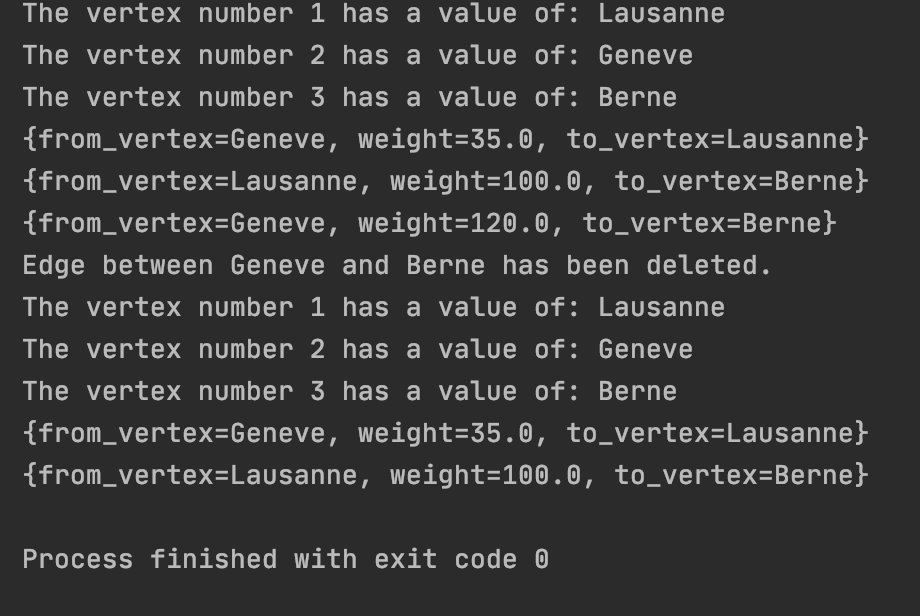
\includegraphics[height=8cm]{ressources/sortie_juste.PNG}

\newpage

\begin{note}{Maeva}
    Ceci devrait être un exercice avancé
\end{note}
\begin{Exercice}[20 minutes]\\

Voici une partie de la classe \lstinline{graph} que vous devez compléter. Implémentez les méthodes \lstinline{update_weight()}, \lstinline{new_edge()} et \lstinline{edge_exist()}.

         \lstinputlisting{ressources/graph_empty.java}
    \begin{enumerate}
        \item La méthode \lstinline{update_weight()} doit prendre en paramètres: le \lstinline{sommet} d'origine, le \lstinline{sommet} d'arrivée ainsi que le poids d'une \lstinline{arête}. Si cette \lstinline{arête} existe alors elle change son poids. Sinon, elle affichera une phrase indiquant que l'\lstinline{arête} n'existe pas.
        \item La méthode \lstinline{edge_exist()} prendra en paramètre le \lstinline{sommet} d'origine et le \lstinline{sommet} d'arrivée. Si cette \lstinline{arête} est dans le \lstinline{graph} alors la méthode renvoie son poids, sinon, elle renvoie 0.
        \item La méthode \lstinline{new_edge} doit créer une instance de \lstinline{Edge} et l'ajouter à l'ensemble \lstinline{edges} si la connexion n'existe pas déjà. Si elle existe avec un autre poids mettre à jour le poids. Si elle existe de façon identique alors retournez la dans la console en utilisant un \lstinline{System.out.print}. Enfin, si on est dans aucun des deux cas précédents utiliser la méthode \lstinline{generate_edge} qui vous est donnée pour créer et ajouter cette arête au \lstinline{graph}. La méthode \lstinline{new_edge} aura pour paramètres: le \lstinline{sommet} d'origine, le \lstinline{sommet} d'arrivée, le poids.
    \end{enumerate}

    \begin{conseil}
    \begin{enumerate}
    \item Utiliser une boucle \lstinline{for} pour parcourir toutes les \lstinline{arêtes} dans le \lstinline{graph}. Faire un test sur les attributs de \lstinline{Edge} pour changer le poids.
    \item Il faut tester pour chaque \lstinline{arête} ( itération) si elle  est égale à celle donnée en paramètres.
    \item Il faut utiliser les méthodes \lstinline{edge_exist()}, \lstinline{update_edge()} et \lstinline{generate_edge()} pour écrire cette méthode. Il y a 4 tests à effectuer: 
        \begin{enumerate}
        \item Si \lstinline{l'arête} existe.
        \item Si \lstinline{l'arête} existante a le même poids que celle indiquée en paramètre de la méthode.
        \item Si \lstinline{l'arête} existante n'a pas le même poids que celle indiquée en paramètre de la méthode.
        \item Utilisez le résultat de \lstinline{edge_exist} pour simplifier ces tests.
        \end{enumerate}
    \end{enumerate}
    \end{conseil}
    \begin{solution}
    \textbf{Java :}
         \lstinputlisting{solutions/Edge.java}
    \end{solution}
    \begin{solution}
    \textbf{Java :}
         \lstinputlisting{solutions/graph1.java}
    \end{solution}
    % TODO: Découper les fichiers de solutions pour qu'ils tiennent sur une page. Les renommer graph_1.java, graph_2,java par exemple et les mettre dans un dossier "Display" ou "Affichage". Mettre le fichier complet dans le dossier solution.
    \begin{solution}
    \textbf{Java :}
         \lstinputlisting{solutions/graph2.java}
    \end{solution}

\end{Exercice}

\newpage

\end{document}
